\documentclass[a4paper,12pt]{article}
\addtolength{\oddsidemargin}{-1.cm}
\addtolength{\textwidth}{2cm}
\addtolength{\topmargin}{-3cm}
\addtolength{\textheight}{3.5cm}
\makeindex


\usepackage[pdftex]{graphicx}
\usepackage{makeidx}
\usepackage{float}
\usepackage{hyperref}
\hypersetup{
	colorlinks=true,
	linkcolor=blue,
	filecolor=magenta,      
	urlcolor=cyan,
}



% define the title
\author{CodeBlox}
\title{Tender}
\begin{document}
	\setlength{\parskip}{6pt}
	
	% generates the title
	\begin{titlepage}
		\begin{center}
			
\includegraphics[width=1\textwidth]{./Pictures/up_logo.png}\\[1.5cm] 
			\textsc{\LARGE Department of Computer Science} \\ [.5cm]
			\textsc{\Large Unit Test Plan and Report} \\ [.5cm]
			\line(1,0){450}\\[.5cm]
			\huge{\bfseries Client: Gavin Potgieter}\\
			\line(1,0){450}\\[.5cm]
			\textsc{\LARGE Team: CodeBlox}\\ [0.5cm]
			
			
			\textsc{\large Lethabo Mogase (Bsc: Computer Science)}\\
			\textsc{\large Lorenzo Spazzoli (Bsc: Computer Science)}\\
			\textsc{\large Bilal Muhammad (BIS: Multimedia)}\\
			\textsc{\large Dirk de Klerk (BIS: Multimedia)}\\ [3.9cm]
			
			\large\today
		\end{center}
	\end{titlepage}
	
	\tableofcontents
	\thispagestyle{empty}
	\footnotesize
	\normalsize
	
	
	
	
	\newpage
	\section{Introduction}
		\subsection{Purpose}
		The main objective of this system is to allow a delivery person into a demarcated area of your house when you are not there. You should be able to give access remotely and monitor the delivery person while you they are in the area.
		
		This document will demonstrate how the functionality of this system was tested by team codeBlox
		
		\subsection{Scope}
		The scope of this document is structured as follows. The features that are considered for testing are listed in section *INSERT SECTION NUMBER*. Tests that have been identified from the requirements are discussed in detail in section *INSERT SECTION NUMBER* Furthermore, this document outlines the test environment and the risks involved in the testing approaches that will be followed. Assumptions and dependencies of this test plan will also be mentioned. Section*INSERT SECTION NUMBER* outlines, discusses and concludes on the results of the tests, respective
		
		\subsection{Test Environment}
			\begin{itemize}
				\item Programming Language
					\begin{itemize}
						\item node js
						\item Angular js
						\item Python
						\item Java (android)
					\end{itemize}
			
			\item Coding Environment
				\begin{itemize}
					\item Node package envrionment (npm)
				\end{itemize}
		
			\item Operating system
				\begin{itemize}
					\item Linux
				\end{itemize}
		
			\item Hardware
				\begin{itemize}
					\item Hardware testing is done on a level of using a voltameter
					\item Raspberry Pi 3
				\end{itemize}
		\end{itemize}
	
	\subsection{Assumption and Dependencies}
		\begin{itemize}
			\item assume that user has android device and is able to use it
			\item assume that the Pi 3 and camera have been setup in the house
		\end{itemize}
		
		\subsubsection{Dependencies}
			\begin{itemize}
					\item angular
					\item bcrypt
					\item body-parser
					\item express
					\item jwt-simple
					\item mongojs
					\item mocha
					\item should
					\item supertest
			\end{itemize}
			
			all npm node-modules
\section{Test Items}
	\section{Functional Features to be Tested}
		\begin{itemize}
				\item user registration
				\item notification when someone is at the gate
				\item open/close gate
				\item open camera
		\end{itemize}
		
		
		\begin{tabular}{c c c c}
			Feature ID & RDS source & Summary & Test Case ID\\ [0.5ex]
			\hline
			
			1 & server.get('/')& Passed & 001 \\
			2 & server.post('/registration') & Passed & 002 \\
			3 & server.get('/returnUser/:email') & Passed & 003 \\
			4 & newUser.getActivationStatus() & Passed & 004 \\
			5 & newUser.getPin() & Passed & 005 \\
			6 & newUser.getStaus() & Passed & 006 \\
		\end{tabular}
	\section{Test Cases}
		\subsection{Test Case 1}
		Test case 1: connection to server \newline
		condition: open home page \newline
		objective: check if the Pi connects to the server \newline
		Input: web URL \newline
		Outcome:  200 status \newline
		
	\subsection{Test Case 2}
		Test case 2: add user \newline
		condition:  user should not exist \newline
		objective: check if user details get persisted to the database
		Input: first name, last name, id, email, password1, password2 \newline
		Outcome: 200 status and user added to database \newline
		
		\subsection{Test Case 3}
		Test case 3: getting user email \newline
		condition:  user should exist \newline
		objective: check if user info can be accessed \newline  
		Input: user name \newline
		Outcome: print user email \newline
			
		\subsection{Test Case 4}
		Test case 4: user status \newline
		condition: user should exist and be active \newline
		objective: check if correct status returned is active \newline
		Input: end Activation Date \newline
		Outcome: active \newline
		\newline
		condition2: user should exist and be inactive \newline
		objective: check if correct status returned is inactive \newline
		Input: end Activation Date \newline
		Outcome: inactive \newline
		
		\subsection{Test Case 5}
		Test case 5: generating pin \newline
		condition: request pin \newline
		objective: generate pin for the back up system \newline
		input: getpin() \newline
		Outcome: 8-digit random pin \newline
		
		\subsection{Test Case 6}
		Test case 6: pin status \newline
		condition: pin has been generated and un-used \newline
		objective: check if pin has not been used \newline
		input: getPinStatus() \newline
		Outcome: un-used \newline
	
		condition2: pin has been generated and used
		objective: check if pin has been used
		input: getPinStatus()
		Outcome: used
		
	\section{Item Pass Criteria}
		\begin{itemize}
			\item The home raspberry pi should be running
			\item The raspberry pi should be connected to the internet
			\item The raspberry should have a connection to the server
		\end{itemize}
		
	\section{Test Deliverables}
	
	\section{Detailed Test Results}
		\subsection{Overview of Test Results}
		All the tests that were carried out passed and meet the expected results. These tests were carried out using the Mocha framework along with an assertion library called Chai.
		
		\subsection{Functional Requirements Test Results}
		Two separate tests were carried out to ensure that everything works. The first set of tests were done over the internet to ensure connection to server and correct communication with the server. The second set of tests, tested the functionality of the individual functions in the module locally. The tests are on Github at :https://github.com/billibongers/CodeBlox---Main-Project/tree/master/Code/Interfaces/tests and https://github.com/billibongers/CodeBlox---Main-Project/tree/master/Code/NodeJs/Services/personModule/test 
		
			\subsubsection{Test Case 1 (4.1)}
			The website opened and the video stream started \newline
			Result \newline
			Pass \newline
			
			\subsubsection{Test Case 2 (4.2)}
			New user was added to the system \newline
			server returned status code of 200 \newline
			Result \newline
			Pass \newline
			
			\subsubsection{Test Case 3 (4.3)}
			User email was returned \newline
			The data was returned in the correct format \newline
			Result \newline
			Pass \newline
			
			\subsubsection{Test Case 4 (4.4)}
			condition 1 returned active and condition 2 returned inactive \newline
			Result \newline
			Pass \newline
			
			\subsubsection{Test Case 5 (4.5)}
			Random 8-digit pin was created
			the pin was returned in the correct format \newline
			pin was linked to correct user \newline
			Result \newline
			Pass \newline
			
			\subsubsection{Test Case 6 (4.6)}
			Condition 1 returned un-used status and condition 2 returned used status \newline
			Result \newline
			Pass \newline
	
	\section{Other}
	Picture of running tests \newline
				
\includegraphics[width=1\textwidth]{./Pictures/1.png}\\[1.5cm] \newline
				
	picture of unit test code \newline
				
\includegraphics[width=1\textwidth]{./Pictures/2.png}\\[1.5cm] \newline
				
				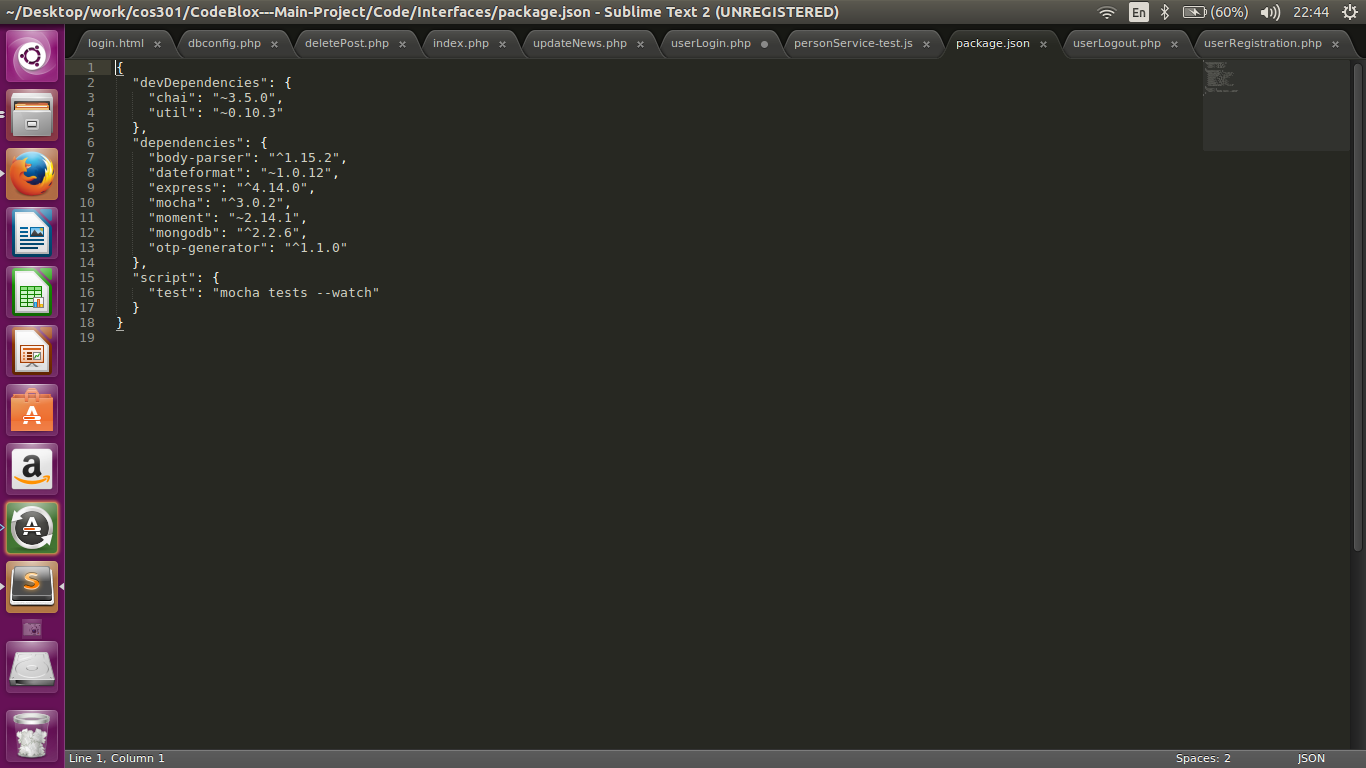
\includegraphics[width=1\textwidth]{./Pictures/3.png}\\[1.5cm] \newline
				
	\section{Conclusions and Recommendations}
	We have gained much insight in terms of testing and its uses. We switched to a testing strategy called Test Driven Development, hereto referred as TTD. With TTD, we are able to write tests without any code written to pass it. This enables the user to write unbiased code because we have no knowledge of the inner code. 
	
	We have also learnt to write tests that test a function in depth. This was achieved by using a special library called chai that is used in conjunction with mocha. It has a vast library of asserts that can be used.
	
	Overall, we are happy with our progress as far as testing is concerned. After completion, if time allows, we wish to carry out a usability test.
				
			
			
			
			
			
		
		
		
		
		
\end{document}
		
		